\newpage
\section{Generating and collecting synthetic data}
\label{s:DataGAGeneration}
\label{s:DataGeneration}


Management of each worker is conducted from the scanner host, as this is the host initiating the scanning tasks.
The task issuing is conducted through a Bash script described in section \ref{s:ScannerScript}.

\begin{figure}[htbp]
\centerline{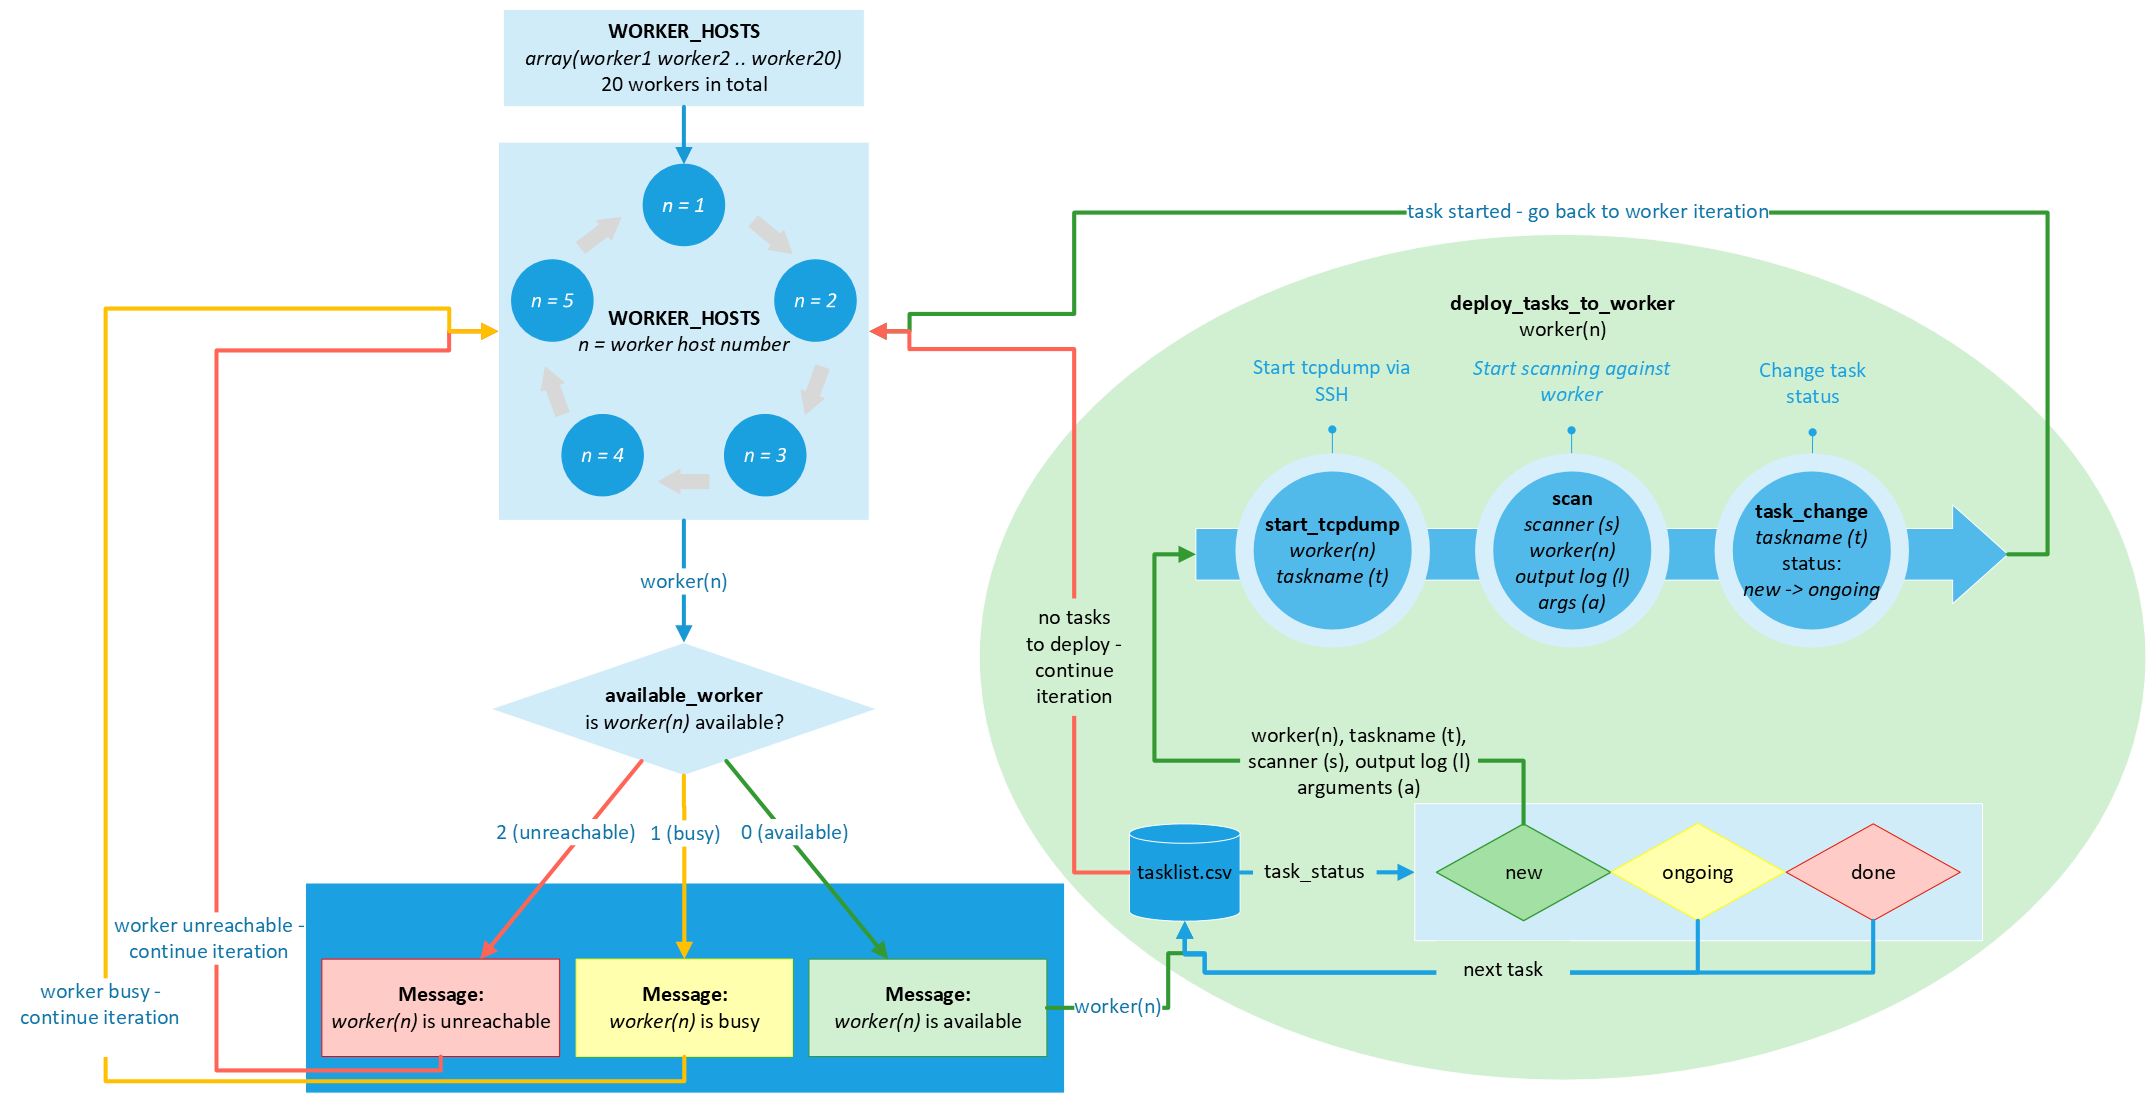
\includegraphics[scale=0.43]{images/lab/ScannerFlowChart.png}}
\caption{Scanning environment flow chart}
\label{fig:ScannerFlowChart}
\end{figure}

As seen in figure \ref{fig:ScannerFlowChart} an array containing all the worker's hostname are enlisted as $WORKER\_HOSTS$.
This is an input to the loop seen below, also marked as $WORKER\_HOSTS$, and $n$ is defined as the identification number for each worker host.
The array is iterated, starting on $worker1$ where the function $available\_worker$ checks if the given worker is available.
An error code is returned as the status of the worker. If the worker is unreachable, code $2$ is returned, and a message is printed saying the worker is unreachable.
If the worker is busy, code $1$ is returned, and a message is printed saying the worker is busy.
With the given error code $1$ or $2$, the iteration in the loop is continued with an increment of the number with $+1$, and the mentioned process is repeated with the worker now set to $worker2$.
When the $available\_worker$ function finds an available worker, it returns a $0$ error code and returns a message informing the availability of a worker.
Now a new iteration in function $deploy\_tasks\_to\_worker$, code shown in listing \ref{lst:DeployTaskWorker}, are started.
It iterates through each line in the tasklist, checking the status of the given task. If the given task is either \textit{ongoing} or \textit{done} it continues the iteration until it finds a task with the status \textit{new}. If a task is found with the status \textit{new} the script starts tcpdump on the worker with the given task name. Then it starts the scan on the scanning host towards the given work with the scanner arguments. Further it changes the status for the task from \textit{new} to \textit{ongoing}.
The iteration of workers now continues until it reaches the last worker, which in this research is $worker20$.
During the research, this script has been run as a cronjob with the entry shown in \ref{lst:ScannerCronJob}.
This cronjob is configured to run each \nth{3} minute. To edit a cronjob, run the command $crontab$ $-e$ as root on the scanner host.

\begin{listing}[!ht]
\caption{Cronjob entry for running scanner each third minute}
\label{lst:ScannerCronJob}
\begin{minted}{Bash}
*/3 * * * * /bin/bash /root/scan.sh tasklist.csv > /dev/null 2>&1
\end{minted}
\end{listing}
It can also be executed manually, and the same operations will be conducted.
The task list is enlisted in a comma-separated file for enhanced readability for the user populating the task list, as seen in figure \ref{fig:LabTasklist}.

\begin{figure}[htbp]
\centerline{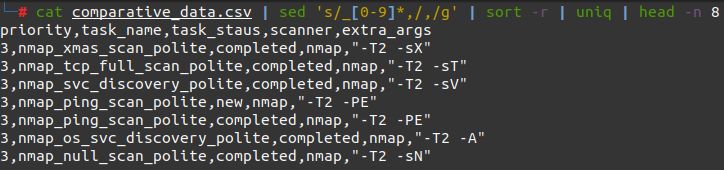
\includegraphics[scale=0.5]{images/lab/tasklist.png}}
\caption{Capture of task list.}
\label{fig:LabTasklist}
\end{figure}

During this process, a task manager described in \ref{ss:Cleanup}, is maintaining the tasklist changing the status on ongoing tasks to complete when they finish.
Within this process, the running tcpdump on the worker is terminated, and the tasklist is updated with the correct status.
This is an iterative process that requires the script to be manually executed and runs until it is terminated either by a user or unexpectedly.

These are the two most important components of the framework.
Additional components are created to efficiently populate a new tasklist from a template tasklist described in listing \ref{lst:TaskPopulation}, and a monitoring component which shows details of a running task shown in figure \ref{fig:LabScanMonitor}.
